\section{Replication}
\label{sec:cryptobinary-replication}

We now undertake a comprehensive replicability evaluation of existing work across different categories of cryptographic algorithms with our newly proposed analysis framework, in order to understand their consistency, robustness, and effectiveness. Our replication evaluation follows the ACM guidelines on replicability \cite{rar}. We rebuild each tool (if the source code is available) and run it across different system environments using our newly developed evaluation benchmark as the test cases\footnote{For the precise details and steps of our replicability evaluation see Appendix \ref{app:cryptobinary-repli_procedure}.}.
This evaluation encompasses all work across this domain, allowing us to delve into their performance and potential limitations. For each cryptographic algorithm, we considered different optimization/obfuscation levels, compilers, and implementations. These experiments are designed to help us understand the consistency and robustness of existing work and techniques, the current status of cryptographic function detection performance and to explore potential future research questions, as well as to highlight existing challenges in cryptographic function detection.  We also involve micro-benchmarks, libraries, and large scale projects to examine each tool's performance in real-world applications.
We present the full results of our evaluation in Table~\ref{tab:cryptobinary-benchmarks} in Appendix~\ref{app:cryptobinary-addltables}, and discuss a selection of the results, as well as their implications, now.

Based on our replicability evaluation, we find that some tools cannot be replicated with our framework. We also highlight some interesting new results, which may help direct future research in this field. This will be addressed in both this section and in Section \ref{sec:cryptobinary-discussion}.


\subsection{Non-Replicable Tools}

\parhead{Aligot} is a cryptographic function identification tool developed based on Pin, a dynamic binary instrumentation framework developed by Intel. We successfully reproduce the test cases that Aligot provided. However, Aligot was tested with Pin 2.10 and Pin 2.12 by its developer, but unfortunately, these versions are no longer available. Consequently, we attempted to use an older version of Pin (3.22) but we were unable to execute Aligot correctly. We believe this to be due to the fact that this tool does not support and cannot be executed on recent CPU architectures.



% \begin{table}[]
% \footnotesize
% \centering
% \begin{tabular}{|cl||c|c|c|c|c|c|c|}
% \hline
% \multicolumn{2}{|c||}{Tool} & \rotatebox[origin=c]{90}{CryptoKnight} & \rotatebox[origin=c]{90}{DRACA} & \rotatebox[origin=c]{90}{Findcrypt2} & \rotatebox[origin=c]{90}{HCD} & \rotatebox[origin=c]{90}{PEiD KANAL} & \rotatebox[origin=c]{90}{SignSrch} & \rotatebox[origin=c]{90}{Where's Crypto} \\ \hline\hline
% \multicolumn{1}{|l|}{\multirow{8}{*}{Algorithm}} & AES & {\color{green}\CIRCLE} & {\color{red}\warn} & {\color{red}\warn} &  &  & {\color{green}\CIRCLE} & {\color{green}\CIRCLE} \\ \cline{2-9} 
% \multicolumn{1}{|l|}{} & DES &  & {\color{red}\warn} & {\color{green}\CIRCLE} &  &  & {\color{red}\warn} & {\color{green}\CIRCLE} \\ \cline{2-9} 
% \multicolumn{1}{|l|}{} & MD5 & {\color{red}\warn} & {\color{green}\CIRCLE} & {\color{green}\CIRCLE} &  &  & {\color{green}\CIRCLE} & {\color{green}\CIRCLE} \\ \cline{2-9} 
% \multicolumn{1}{|l|}{} & RC4 & {\color{red}\warn} &  &  &  &  &  &  \\ \cline{2-9} 
% \multicolumn{1}{|l|}{} & RC5 &  & {\color{green}\CIRCLE} & {\color{green}\CIRCLE} &  &  & {\color{green}\CIRCLE} &  \\ \cline{2-9} 
% \multicolumn{1}{|l|}{} & RSA & {\color{green}\CIRCLE} &  &  &  &  &  &  \\ \cline{2-9}
% \multicolumn{1}{|l|}{} & SHA-1 &  & {\color{green}\CIRCLE} & {\color{green}\CIRCLE} &  &  & {\color{green}\CIRCLE} & {\color{green}\CIRCLE} \\ \cline{2-9} 
% \multicolumn{1}{|l|}{} & SHA-256 &  &  & {\color{green}\CIRCLE} &  &  & {\color{green}\CIRCLE} & {\color{green}\CIRCLE} \\ \cline{2-9} 
% \multicolumn{1}{|l|}{} & TEA &  & {\color{green}\CIRCLE} &  &  &  & {\color{green}\CIRCLE} & {\color{green}\CIRCLE} \\ \hline

% \end{tabular}
% \caption{Comparison}
% \label{tab:comparison}
% \end{table}



% \begin{table}[]
% \begin{tabular}{|l|lllllllll|}
% \hline
% \multirow{2}{*}{Tool} & \multicolumn{9}{l|}{Algorithm} \\ \cline{2-10} 
%  & \multicolumn{1}{l|}{TEA} & \multicolumn{1}{l|}{RC4} & \multicolumn{1}{l|}{RC5} & \multicolumn{1}{l|}{DES} & \multicolumn{1}{l|}{AES} & \multicolumn{1}{l|}{SHA-1} & \multicolumn{1}{l|}{SHA-256} & \multicolumn{1}{l|}{MD5} & RSA \\ \hline
% DRACA & \multicolumn{1}{l|}{{\color{green}\cmark}} & \multicolumn{1}{l|}{} & \multicolumn{1}{l|}{{\color{green}\cmark}} & \multicolumn{1}{l|}{{\color{red}\warn}} & \multicolumn{1}{l|}{{\color{green}\cmark}} & \multicolumn{1}{l|}{{\color{green}\cmark}} & \multicolumn{1}{l|}{} & \multicolumn{1}{l|}{{\color{green}\cmark}} &  \\ \hline
% Findcrypt2 & \multicolumn{1}{l|}{} & \multicolumn{1}{l|}{} & \multicolumn{1}{l|}{{\color{green}\cmark}} & \multicolumn{1}{l|}{{\color{green}\cmark}} & \multicolumn{1}{l|}{{\color{red}\warn}} & \multicolumn{1}{l|}{{\color{green}\cmark}} & \multicolumn{1}{l|}{{\color{green}\cmark}} & \multicolumn{1}{l|}{{\color{green}\cmark}} &  \\ \hline
% HCD & \multicolumn{1}{l|}{} & \multicolumn{1}{l|}{} & \multicolumn{1}{l|}{} & \multicolumn{1}{l|}{} & \multicolumn{1}{l|}{} & \multicolumn{1}{l|}{} & \multicolumn{1}{l|}{} & \multicolumn{1}{l|}{} &  \\ \hline
% PEiD KANAL & \multicolumn{1}{l|}{} & \multicolumn{1}{l|}{} & \multicolumn{1}{l|}{} & \multicolumn{1}{l|}{} & \multicolumn{1}{l|}{} & \multicolumn{1}{l|}{} & \multicolumn{1}{l|}{} & \multicolumn{1}{l|}{} &  \\ \hline
% SignSrch & \multicolumn{1}{l|}{{\color{green}\cmark}} & \multicolumn{1}{l|}{} & \multicolumn{1}{l|}{{\color{green}\cmark}} & \multicolumn{1}{l|}{{\color{red}\warn}} & \multicolumn{1}{l|}{{\color{red}\warn}} & \multicolumn{1}{l|}{{\color{green}\cmark}} & \multicolumn{1}{l|}{{\color{green}\cmark}} & \multicolumn{1}{l|}{{\color{red}\warn}} &  \\ \hline
% CryptoKnight & \multicolumn{1}{l|}{} & \multicolumn{1}{l|}{{\color{red}\warn}} & \multicolumn{1}{l|}{} & \multicolumn{1}{l|}{} & \multicolumn{1}{l|}{{\color{green}\cmark}} & \multicolumn{1}{l|}{} & \multicolumn{1}{l|}{} & \multicolumn{1}{l|}{{\color{red}\warn}} & {\color{green}\cmark} \\ \hline
% Where's Crypto & \multicolumn{1}{l|}{{\color{green}\cmark}} & \multicolumn{1}{l|}{} & \multicolumn{1}{l|}{} & \multicolumn{1}{l|}{{\color{green}\cmark}} & \multicolumn{1}{l|}{{\color{green}\cmark}} & \multicolumn{1}{l|}{{\color{green}\cmark}} & \multicolumn{1}{l|}{{\color{green}\cmark}} & \multicolumn{1}{l|}{{\color{green}\cmark}} &  \\ \hline
% \end{tabular}
% \label{tab:comparison}
% \caption{Comparison}
% \end{table}



% \subsection{Benchmark Evaluation}
% We firstly evaluate these tool with cryptographic function in our new developed benchmark. We do find some previous evaluate result that cannot be reproduce, which has been introduce in \autoref{subsec:unreproduce}

% In our micro-benchmark evaluation, we also find some false positive result. None of the tool falsely consider file handle, I/O, network connection, or heave math operation as cryptographic function. However, CryptoKnight and Signsrch miss claim a mathematical matrix as cryptographic function such as AES. AES algorithm has Rijndael S-box, so cryptographic function detection tool with static signature search approach may false reconazation a matrix as AES function.

% Finally, besides the standard cryptographic function, we also select some crypthrapgic. We find that many tool detect cryptographic function from these libraries since some of these libraries such as openssl and libgcrypt do have cryptographic function in the binary. However, some tool cannot correctly detect cryptographic function in real world applications 
% For example, DRACA, HCD, and Signsrch cannot detect any cryptographic function from openssl; CryptoKnight and HCD cannot detect cryptographic function from libgcrypt etc.

\subsection{Unexpected Detection Results}
\label{subsec:cryptobinary-false}

\begin{table}[]
\footnotesize
\centering
\begin{adjustbox}{max width=\textwidth}
\begin{tabular}{c||c|c|c|c|c|c|c|c|c}
\hline
\multirow{2}{*}{Tool} & \multicolumn{9}{c}{Cryptographic Algorithm} \\ \cline{2-10}
& AES & DES & MD5 & RC4 & RC5 & RSA & SHA1 & SHA256 & TEA \\ \hline
\hline
DRACA & \xmark & \xmark & \cmark &  & \cmark &  & \cmark &  & \cmark \\ \hline
CryptoKnight & \cmark &  & \xmark & \xmark &  & \cmark &  &  &  \\ \hline
FindCrypt2 & \xmark & \cmark & \cmark &  & \cmark &  & \cmark & \cmark & \cmark \\ \hline
HCD         & \textminus & \textminus & \textminus & \textminus & \textminus & \textminus & \textminus & \textminus & \textminus \\ \hline
PEiD KANAL & \textminus & \textminus & \textminus & \textminus & \textminus & \textminus & \textminus & \textminus & \textminus \\ \hline
SignSrch & \cmark & \xmark & \cmark &  & \cmark &  & \cmark & \cmark & \cmark \\ \hline
Where's Crypto & \cmark & \cmark & \cmark &  &  &  & \cmark & \cmark & \cmark \\ \hline
\end{tabular}
\end{adjustbox}
\caption{Comparative analysis of detection approaches versus stated capabilities in original documentation. Cross mark denotes inconsistencies (false positive or false negative), check mark successful replication.}
\label{tab:cryptobinary-comparison}
%\vspace{-20pt}
\end{table}

We begin by discussing evaluation results that were either unexpected or inconsistent based on prior stated findings.
During our evaluation, we encountered instances where certain tools yielded false positives or false negatives in their detection outcomes. These findings underline the importance of a more in-depth and rigorous analysis to ensure the attainment of dependable detection results. As a result, it is evident that further development is required to enhance reliability.

\parhead{Unreplicable cryptographic function detection.} In \autoref{tab:cryptobinary-summary}, we list the purported performance for each tool. However, our evaluation could not verify the detection capabilities for certain cryptographic functions in some of the tools. \autoref{tab:cryptobinary-comparison} presents the outcomes of our assessment relative to the detection capabilities as claimed by the respective tools' original documentation. If a tool claims to have the ability to detect a cryptographic algorithm, but we cannot reproduce the same result in any of our benchmarks or evaluation metrics, we mark it with a red exclamation mark. Otherwise, if we can confirm the detection ability, we mark it with a green circle. A blank means the tool makes no claim about the given algorithm.  Due to the unavailability of documentation for HCD and PEiD KANAL, a comparison of our evaluation results with their claimed detection capabilities was not possible.

\parhead{Micro-benchmark false positives.} In our micro-benchmark evaluations, we also uncovered new false positive results. None of the tools falsely considered operations like file handling, I/O, network connection, or heavy math operations as cryptographic functions. However, some tools, such as CryptoKnight and Signsrch, mistakenly identify a mathematical matrix as a cryptographic function like AES. Since AES includes the Rijndael S-box (often coded as a matrix), tools that rely on static signature searches may incorrectly recognize a matrix as an AES function. This highlights the importance of broader and more standardized test cases as well, as things like this were not considered by previous evaluations.
To better understand these results, in Table \ref{tab:cryptobinary-quat} (Appendix~\ref{app:cryptobinary-addltables}) we present the detailed breakdown of percentage of false positives and false negatives observed for each tool across various cryptographic functions, offering a comprehensive comparison of their performance in these error metrics. This allows us to gain insight into the likelihood of a tool raising errors when attempting to detect specific cryptographic functions.

\parhead{Undetected cryptographic functions in libraries.} Finally, besides standard stand-alone cryptographic functions, we also selected some real-world cryptographic libraries and libraries with similar behavior to cryptographic functions to test on. We find that many tools successfully detect cryptographic functions in these libraries, which is expected, as some, including openssl and libgcrypt, are indeed primarily cryptographic libraries.
However, it is interesting to note that this is not true of all tools.  Some work fails to detect cryptographic functions in this setting.  For example, tools like DRACA, HCD, and Signsrch are unable to detect any cryptographic functions from openssl, while CryptoKnight and HCD fail to detect cryptographic functions in libgcrypt. We are not sure why this is the case, and leave this as an interesting avenue for future work.  This also points to the fact that existing work may have unreliable performance in real world (large) programs.

\begin{takeaway}
\textbf{Future Research:} Certain cryptographic-specific libraries seem to pose challenges for existing tools; exploring why this is the case would be an interesting avenue for future work.  Also, existing tools have more false positives/negatives than initially expected, so placing more emphasis on improving detection accuracy and reducing false positives or false negatives seems highly relevant.
\end{takeaway}

% For example, when we carried out our evaluations on a binary that contained RC5, we observed that DRACA, Signsrch, and HCD effectively detected the presence of the RC5 function. However, it is noteworthy that they also identified the TEA function. Both TEA and RC5 belong to the block cipher family, which occasionally leads to the occurrence of false positives and noise in function detection. This situation underscores the importance of exercising caution when a tool identifies multiple cryptographic functions within the same category, as such detections could potentially be false positives resulting from the analysis approaches or weaknesses of the tool itself.

% We also observed instances where certain tools produced false negatives. Some tools claimed to have the capability to detect specific algorithms, but we were unable to reproduce these results. Based on the full evaluation results in Table \ref{tab:benchmarks}, it is evident that AES and DES cannot be detected by many tools, even though many of them should theoretically have the ability to do so.

\subsection{Operating System Limitations}

The usage of certain tools may be constrained by their exclusive compatibility with specific operating systems, impacting their efficacy and analysis capabilities. Many tools are designed and built with specific operating systems in mind.  Fortunately, with the help of other tools, such as WineHQ, which enables software developed for Microsoft Windows to run on Unix-like operating systems, developers can for example use some Windows cryptographic detection tools in Linux. However, tools are not just limited to running on specific operating systems, but also restricted to handling binaries compiled for selected operating systems.
These inherent limitations potentially reduce the scope and depth of analysis a tool can provide, depending on the operating system selected and targeted in the original work.

%For example, most malware is designed for a specific operating system. In order to detect malware and its related cryptographic functions, a developer has to use a cryptographic detection tool that supports the target operating system, or otherwise, such analysis will be hampered.

In Table \ref{tab:cryptobinary-system}, we evaluate the capability of exisiting work to analyze binaries across three different operating systems and for binaries compiled specifically for each of these operating systems. We use a \LEFTcircle \space to indicate cases where a tool cannot be executed on a Unix-like system but becomes functional with the assistance of WineHQ.

\begin{takeaway}
\textbf{Takeaway:} Ideally cryptographic function detection tools need to support all operating systems to effectively detect cryptographic functions or malware across diverse environments and improve overall detection measures.
\end{takeaway}

% Please add the following required packages to your document preamble:
% \usepackage{multirow}
%\vspace*{-10pt}
\begin{table}[t]
\centering
\begin{adjustbox}{max width=\textwidth}
\begin{tabular}{c||ccc||ccc}
\hline
\multirow{2}{*}{Tool} & \multicolumn{3}{c||}{Supported System}                               & \multicolumn{3}{c}{Supported Binary}                               \\ \cline{2-7} 
                      & \multicolumn{1}{c|}{Windows} & \multicolumn{1}{c|}{macOS} & Linux & \multicolumn{1}{c|}{Windows} & \multicolumn{1}{c|}{macOS} & Linux \\ \hline \hline
Aligot                & \multicolumn{1}{c|}{\CIRCLE}       & \multicolumn{1}{c|}{\CIRCLE}     & \CIRCLE     & \multicolumn{1}{c|}{\CIRCLE}       & \multicolumn{1}{c|}{\CIRCLE}     & \CIRCLE     \\ \hline
CryptoHunt            & \multicolumn{1}{c|}{\Circle}       & \multicolumn{1}{c|}{\Circle}     & \CIRCLE     & \multicolumn{1}{c|}{\Circle}       & \multicolumn{1}{c|}{\Circle}     & \CIRCLE     \\ \hline
CryptoKnight          & \multicolumn{1}{c|}{\CIRCLE}       & \multicolumn{1}{c|}{\CIRCLE}     & \CIRCLE     & \multicolumn{1}{c|}{\CIRCLE}       & \multicolumn{1}{c|}{\CIRCLE}     & \CIRCLE     \\ \hline
DRACA                 & \multicolumn{1}{c|}{\CIRCLE}       & \multicolumn{1}{c|}{\LEFTcircle}     & \LEFTcircle     & \multicolumn{1}{c|}{\CIRCLE}       & \multicolumn{1}{c|}{\CIRCLE}     & \CIRCLE     \\ \hline
FindCrypt2            & \multicolumn{1}{c|}{\CIRCLE}       & \multicolumn{1}{c|}{\CIRCLE}     & \CIRCLE     & \multicolumn{1}{c|}{\CIRCLE}       & \multicolumn{1}{c|}{\CIRCLE}     & \CIRCLE     \\ \hline
HCD                   & \multicolumn{1}{c|}{\CIRCLE}       & \multicolumn{1}{c|}{\LEFTcircle}     & \LEFTcircle     & \multicolumn{1}{c|}{\CIRCLE}       & \multicolumn{1}{c|}{\Circle}     & \Circle     \\ \hline
Kerckhoff             & \multicolumn{1}{c|}{\CIRCLE}       & \multicolumn{1}{c|}{\Circle}     & \Circle     & \multicolumn{1}{c|}{\CIRCLE}       & \multicolumn{1}{c|}{\Circle}     & \Circle     \\ \hline
PEiD KANAL            & \multicolumn{1}{c|}{\CIRCLE}       & \multicolumn{1}{c|}{\LEFTcircle}     & \LEFTcircle     & \multicolumn{1}{c|}{\CIRCLE}       & \multicolumn{1}{c|}{\CIRCLE}     & \CIRCLE     \\ \hline
Signsrch              & \multicolumn{1}{c|}{\CIRCLE}       & \multicolumn{1}{c|}{\LEFTcircle}     & \LEFTcircle     & \multicolumn{1}{c|}{\CIRCLE}       & \multicolumn{1}{c|}{\CIRCLE}     & \CIRCLE     \\ \hline
Where’s Crypto        & \multicolumn{1}{c|}{\CIRCLE}       & \multicolumn{1}{c|}{\Circle}     & \Circle     & \multicolumn{1}{c|}{\CIRCLE}       & \multicolumn{1}{c|}{\CIRCLE}     & \CIRCLE     \\ \hline
\end{tabular}
\end{adjustbox}
\caption{Tool compatibility with different operating systems; \CIRCLE represents a tool that supports the desired system, while \Circle indicates a tool that does not support the desired system; \LEFTcircle \space represents cases where a tool cannot be executed on a Unix-like system but becomes functional with the assistance of WineHQ}
\label{tab:cryptobinary-system}
\vspace*{-10pt}
\end{table}


% \section{Evaluation}
% \label{sec:evaluation}
% \fanyo{Beside the general future research focusing directions such as improving accuracy, reducing false positive, and/or supporting more cryptographic function, we also propose some future research questions that are significant importance for this fields}

% We now undertake a comprehensive evaluation of different tools across different categories of cryptographic algorithms in order to understand their effectiveness.
% This evaluation encompasses both earlier iterations and the most recent developments in this domain, allowing us to delve deep into their performance and potential limitations.
% For each algorithm, we considered different optimization/obfuscation levels, compilers, and implementations. These experiments are designed to explore and evaluate our proposed research questions, as well as to highlight existing challenges in cryptographic function detection.
% We present the full results of our evaluation in Table~\ref{tab:benchmarks} in Appendix~\ref{app:addltables}, and discuss a selection of the results, as well as their implications, now.
% Note that for various reasons, we were unable to run and evaluate some of tools with our full benchmarking framework and evaluation metrics. These issues are discussed in Appendix \ref{subsec:unavailable}.




% Table \ref{benchmarks} shows  evaluation results for each tool we select. Checkmark represents that the tool detects cryptographic algorithm in the binary program, and cross represents that no cryptographic algorithm is found. There are some notes for the evaluation results in the table.

% \begin{itemize}[leftmargin=*]
%     \setlength{\itemsep}{0pt}
%     \setlength{\parskip}{0pt}
%         \item $+$: There are more than one cryptographic algorithms are detected by the tool.
%         \item $\times$: False negative - tool should but cannot detect the cryptographic algorithms.
%         %\item $B$: Signsrch recognize bzip2 binary since bzip2 has a specific signature that Signsrch supported.
% \end{itemize}

% Next, we analyze the evaluation results in multiple directions with selected cryptography detection tools and algorithms. Full evaluation results for all tools and benchmarks will be shown in Table \ref{benchmarks}. 


\subsection{Impact of Compiler Variations}
\label{subsec:cryptobinary-effect-compiler}

%\emph{R1: Does the choice of compiler play a role in the detection success?}

To study the impact of compilers on cryptographic function detection, we compiled each program in our benchmarking framework with GCC/G++, CLANG/CLANG++, and MSVC.  Somewhat as expected given the impact a compiler can have on the resulting binary, our evaluation shows that tools may output quite different results for different compilers.  We choose MD5 as an illustrative example, shown in Figure \ref{fig:cryptobinary-evaluate_compiler}, though we have observed the same general trends across most cryptographic schemes.

\begin{figure}[ht]
    \centering
  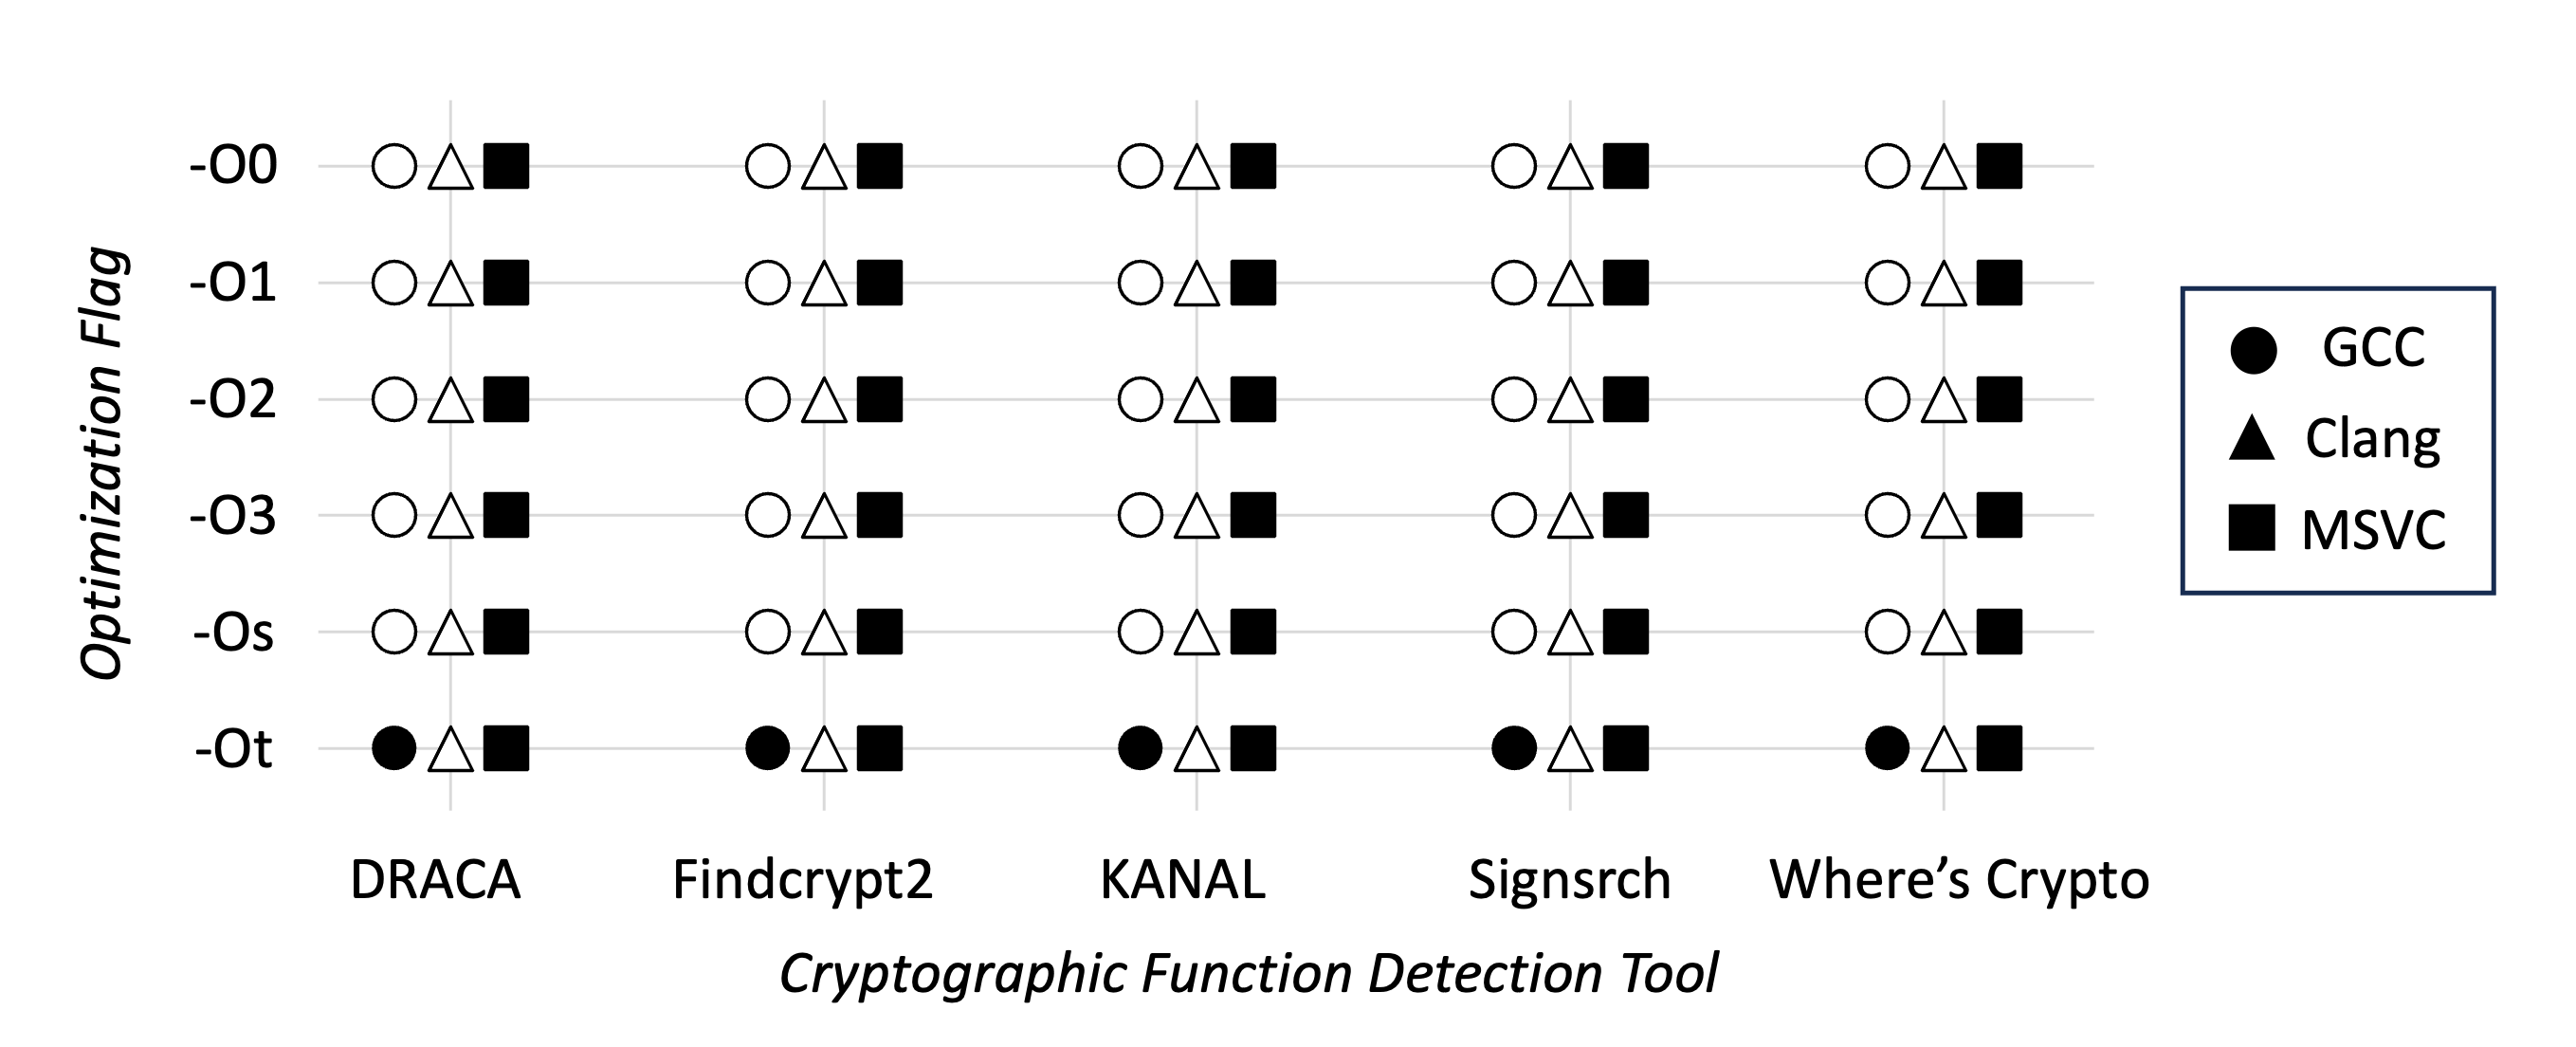
\includegraphics[width=0.8\linewidth,keepaspectratio]{ch-cryptobinary/figure/evaluate_compiler_new.png}
	%\vspace*{-10pt}
  \caption{Evaluation result for MD5 with different compilers. A full marker indicates that function can be detected and an empty marker that it cannot.}
  \label{fig:cryptobinary-evaluate_compiler}
\end{figure}

\fanyo{fix typo in figure!!!}

In this example, DRACA, Findcrypt2, PEiD KANAL, Signsrch, and Where's Crypto support detecting the MD5 algorithm. However, their detection capabilities are influenced by the compiler used. All of these tools can detect the MD5 algorithm in binaries compiled with the MSVC compiler, regardless of the optimization flag. In contrast, for binaries compiled with GCC, they can only detect the MD5 algorithm when the -O0 optimization flag is applied. Furthermore, when using the Clang compiler, none of these tools were able to detect the MD5 algorithm in the binary. This suggests that differences between compilers may significantly impact a tool's analysis results. In general, we found that the MSVC compiler has less impact on detection results compared to GCC and CLANG. Specifically, if a tool can detect a certain cryptographic algorithm in a program compiled by GCC or CLANG, it will also be able to detect that algorithm in the same program compiled by MSVC.

For example, Signsrch shows inconsistent performance with Clang, GCC, and MSVC, identifying the SHA-1 hash function in certain programs compiled with identical optimization flags but using a different compiler. We also observe same behaviour for DARACA when detect XXTEA algorithm (see Table \ref{tab:cryptobinary-benchmarks} for details).

The structure of binaries produced by different compilers, such as MSVC, GCC, and LLVM, can vary significantly due to differences in object file formats, optimization strategies, and code generation techniques. Binary analysis often relies on symbolic information, padding, and inlined data, all of which are heavily influenced by the compiler version~\cite{andriesse2017compiler}. These variations can hinder the effectiveness of cryptographic function detection tools, potentially leading to inaccurate or incomplete detection results.

%\noindent\fbox{%
    %\parbox{\textwidth}{%
        %Future Research Question: At present, it is notable that none of the cryptographic function detection tools take into account the influence of the compiler. Our evaluation results have revealed that the choice of compiler plays a pivotal role in cryptographic function analysis.
        %%We have identified differences in behavior between standard, widely used compilers like GCC and CLANG. Additionally, other non-standard compilers may introduce even more variations and challenges for cryptographic function detection tools. 
        %The exploration of compiler effects and their incorporation into cryptographic function detection tools represents an enticing avenue for future research, and understanding and accounting for these compiler-related influences could significantly enhance the accuracy and reliability.
    %}%
%}

\begin{takeaway}
\textbf{Future Research:} At present, it is notable that none of the cryptographic function detection tools consider the impact of the compiler. Our evaluation results have revealed that the choice of compiler plays a pivotal role in cryptographic function analysis.
        %We have identified differences in behavior between standard, widely used compilers like GCC and CLANG. Additionally, other non-standard compilers may introduce even more variations and challenges for cryptographic function detection tools. 
        The exploration of compiler effects and their incorporation into cryptographic function detection tools represents an enticing avenue for future research.
        Moreover, understanding and accommodating these compiler-related influences could significantly enhance both accuracy and reliability.
        %and understanding and accounting for these compiler-related influences could significantly enhance accuracy and reliability.
\end{takeaway}


% \begin{table}[h]
% \centering
% \begin{tabular}{|cc|c|c|c|c|}
% \hline
% \multicolumn{2}{|c|}{Binary Prog}                    & DRACA  & Findcrypt2 & PEiD KANAL & Where's Crypto \\ \hline
% \multicolumn{1}{|c|}{\multirow{2}{*}{XXTEA}} & gcc   & \cellcolor{gray!25}\cmark & \cmark     & \cmark     & \cmark         \\ \cline{2-6} 
% \multicolumn{1}{|c|}{}                       & clang & \cellcolor{gray!25}\xmark & \cmark     & \cmark     & \cmark         \\ \hline
% \multicolumn{1}{|c|}{\multirow{2}{*}{MD5}}   & gcc   & \cellcolor{gray!25}\cmark & \cellcolor{gray!25}\cmark     & \cellcolor{gray!25}\cmark     & \cellcolor{gray!25}\cmark         \\ \cline{2-6} 
% \multicolumn{1}{|c|}{}                       & clang & \cellcolor{gray!25}\xmark & \cellcolor{gray!25}\xmark     & \cellcolor{gray!25}\xmark     & \cellcolor{gray!25}\xmark         \\ \hline
% \end{tabular}
% \caption{Untitled}
% \label{tab:evaluate_compiler}
% \end{table}

 %\begin{table}[h]
 %\centering
 %\begin{tabular}{|c|c|c|c|c|c|c|c|c|c|c|c|c|}
 %\hline
 %Flag   & None  & -O0   & -O1   & -O2   & -O3   & -Os   & -Ofast & obs\_sub & obs\_fla & obs\_bcf & Multi\_flag 1 & Multi\_flag 2 \\ \hline
 %Prog 1 & \cmark & \cmark & \cmark & \xmark & \xmark & \xmark & \xmark  & \cmark    & \cmark    & \cmark    & \cmark         & \xmark         \\ \hline
 %Prog 2 & \cmark & \cmark & \xmark & \xmark & \xmark & \xmark & \xmark  & \cellcolor{gray!25} & \cellcolor{gray!25} & \cellcolor{gray!25} & \cellcolor{gray!25} & \cellcolor{gray!25} \\ \hline
 %\end{tabular}
 %\caption{Untitled}
 %\label{tab:evaluate_flag}
 %\end{table}

\subsection{Impact of Optimization Flags}
%\emph{R2: Is there any impact from optimization flags?}

Optimization flags and obfuscation can significantly impact the analysis results for cryptographic functions \cite{ren2021unleashing}. CryptoHunt\cite{xu2017cryptographic} and FALKE-MC \cite{aigner2018falke} have explored this direction. CryptoHunt primarily focuses on specific optimization flags such as \texttt{-O0}, \texttt{-O1}, and \texttt{-O2}, while FALKE-MC includes programs compiled with \texttt{-Os} and \texttt{-Ofast} for training. However, we are unable to run either of these tools, so we cannot confirm their detection performance with optimization/obfuscations flags. In order to comprehensively investigate this topic, we have expanded our study to include additional optimization flags, obfuscation techniques, and their combinations, thereby providing a more thorough exploration of their impact on cryptographic algorithm detection.

Our findings indicate that both optimization flags and obfuscations can affect detection capability. For instance, based on our results in \autoref{tab:cryptobinary-benchmarks}, we can see that Findcrypt2, PEiD KANAL, Signsrch, and Where's Crypto can detect MD5 when compiled without optimization/obfuscation flags or compiled with \texttt{-O1}. However, none of these tools can detect MD5 if the binary program is compiled with advanced optimization/obfuscation flags such as \texttt{-O2}, \texttt{-Ofast}, or \texttt{-obs\_sub}. In addition, we observed that Signsrch exhibits inconsistent performance for SHA-1 or SHA-256, and DRACA shows unstable performance with XTEA and XXTEA when running with optimization or obfuscation flags.
Optimization flags significantly alter the structure and behavior of a binary program by improving performance, reducing size, and modifying control flow. Techniques like function inlining, loop unrolling, and dead code elimination obscure the original source code structure, making it more difficult for analysts to identify cryptographic functions.
% Table \ref{tab:evaluate_flag} shows selected evaluation results of Signsrch with two different experiment. Experiment 1 is a program contains the SHA-1 hash function compiled by CLANG with different optimization flags or obfuscations, while experiment 2 contains the MD5 hash function compiled by GCC with different optimization flags (as the GCC compiler does not support obfuscations).

% \begin{table}[h]
% \vspace*{-6pt}
% \centering
% \footnotesize
% \begin{tabular}{|c||c|c|c|}
% \hline
% Flag          & SHA-1        & MD5                 \\ \hline \hline
% None          & \cmark       & \cmark              \\ \hline
% -O0           & \cmark       & \cmark              \\ \hline
% -O1           & \cmark       & \xmark              \\ \hline
% -O2           & \xmark       & \xmark              \\ \hline
% -O3           & \xmark       & \xmark              \\ \hline
% -Os           & \xmark       & \xmark              \\ \hline
% -Ofast        & \xmark       & \xmark              \\ \hline
% obs\_sub      & \cmark       & \cellcolor{gray!25} \\ \hline
% obs\_fla      & \cmark       & \cellcolor{gray!25} \\ \hline
% obs\_bcf      & \cmark       & \cellcolor{gray!25} \\ \hline
% -obs\_sub, obs\_fla, obs\_bcf & \cmark       & \cellcolor{gray!25} \\ \hline
% -obs\_sub, obs\_fla, obs\_bcf, -O3 & \xmark       & \cellcolor{gray!25} \\ \hline
% \end{tabular}
% %}
% \caption{Evaluation results of Signsrch with different optimization flags}
% \label{tab:evaluate_flag}
% \vspace*{-0.6cm}
% \end{table}

% We discovered that both optimization flags and obfuscations can affect detection, potentially resulting in false negatives (where the binary contains a cryptographic algorithm but the tool cannot detect it). For example, Signsrch successfully detects TEA in Program 1 compiled without any optimization flags or obfuscations. However, with additional optimization flags, Signsrch cannot detect any cryptographic algorithms at all anymore, resulting in false negatives.

% Meanwhile, Signsrch successfully detects MD5 in Program 2 compiled with no optimization flags or -O0, but cannot detect MD5 in the binary compiled with any other optimization flags or obfuscations. We observed the same results when detecting MD5 with other tools. Therefore, we conclude that current cryptographic detection tools may not be able to handle some algorithms, like MD5, if the binary is compiled with advanced optimization flags such as $-O3$.

%\noindent\fbox{%
    %\parbox{\textwidth}{%
        %Future Research Question: Optimization and obfuscation have been noticed by some researchers such as CryptoHunt, a cryptographic detection tool designed for obfuscated binaries. However, the limitation of CryptoHunt, such as slow time performace due to the large trace size, may reduce its applicability such as large scale project.  Given that certain other tools struggle to handle obfuscated binaries in certain algorithms,  we maintain that the exploration of optimization and obfuscation remains an interesting and important future research direction.
    %}%
%}

\begin{takeaway}
\textbf{Future Research:} The effects of optimization and obfuscation have been noted in works such as CryptoHunt, which is designed specifically for obfuscated binaries. However, limitations such as slow performance due to the large trace size, may reduce its applicability for large scale projects. Considering that many tools seem to face challenges with obfuscated binaries, we assert that investigating the effects of optimization and obfuscation continues to be a compelling and critical avenue for future research.
\end{takeaway}

% \begin{figure}
% \centering
% \begin{minipage}{.45\textwidth}
%   \centering
%   \includegraphics[width=\linewidth]{./images/evaluate_algo.jpg}
%   \caption{Untitled}
%   \label{fig:evaluate_algo}
% \end{minipage}%
% \qquad
% \begin{minipage}{.45\textwidth}
%   \centering
%   \includegraphics[width=1.15\linewidth]{./images/evaluate_tool.jpg}
%   \caption{Untitled}
%   \label{fig:evaluate_tool}
% \end{minipage}
% \end{figure}

\subsection{Impact of Different Algorithm Versions}
\label{subsec:cryptobinary-algo-version}
% \begin{figure}[ht]
%   \includegraphics[width=\columnwidth,keepaspectratio]{./images/evaluate_nonstandard.jpg}
%   \caption{Untitled}
%   \label{fig:evaluate_nonstandard}
  
% \end{figure}

%\emph{R5: Is the version of the algorithm significant during detection?}

We also carried out evaluations to determine whether variations in a cryptographic algorithm affects the success of its detection. As a case study, we analyzed different variants of the Tiny Encryption Algorithm (TEA), including standard TEA, XTEA, and XXTEA. While all the tools were able to successfully detect TEA binaries with any of these three variants, we observed some interesting details in the detection results.

\begin{table}[h]
%\vspace{-6pt}
\centering
\begin{tabular}{l||l|l}
\hline
Algorithm & DRACA                                                                      & Signsrch                                                                                   \\ \hline \hline
TEA   & \begin{tabular}[c]{@{}l@{}}* RC5 or RC6 - 50\%\\ ** TEA - 67\%\end{tabular} & \begin{tabular}[c]{@{}l@{}}* TEA1\_DS {[}32.le.4{]}\\ ** TEA encryption/decryption\end{tabular} \\ \hline
XTEA  & \begin{tabular}[c]{@{}l@{}}* RC5 or RC6 - 50\%\\ ** TEA - 34\%\end{tabular} & * TEA1\_DS {[}32.le.4{]}                                                                     \\ \hline
XXTEA & \begin{tabular}[c]{@{}l@{}}* RC5 or RC6 - 50\%\\ ** TEA - 67\%\end{tabular} & * TEA1\_DS {[}32.le.4{]}                                                                     \\ \hline
\end{tabular}
%}
\caption{Output when evaluating DRACA and Signsrch with different variants of TEA}
\label{tab:cryptobinary-evaluate_variant}
%\vspace*{-0.7cm}
\end{table}

For example, as shown in Table \ref{tab:cryptobinary-evaluate_variant}, when using DRACA to analyze binaries containing TEA or XXTEA, the tool provides a confidence score. It tends to determine that a binary program is more likely to contain TEA functions if TEA or XXTEA is present. However, when analyzing binary programs containing XTEA, DRACA may incorrectly identify RC5 or RC6 as being present in 50\% of cases, and TEA functions in only 34\% of cases. In contrast, Signsrch is able to detect TEA functions in all three binary programs containing TEA, XTEA, or XXTEA, but it may identify different TEA signatures in each binary.

%\noindent\fbox{%
    %\parbox{\textwidth}{%
        %Future Research Question: Our evaluations suggests that the variant versions of cryptographic algorithms also play a crucial role in detection, and that cryptographic function detection tools may not be able to accurately detect certain variant algorithms based on their signatures alone. Currently, there is no approach focuses on this difference, which could be a future research path for crytpographic function detection.
    %}%
%}

\begin{takeaway}
\textbf{Future Research:} Our evaluations indicates that the variant or version of a cryptographic algorithm plays a crucial role in its detection, suggesting that existing tools might struggle to accurately identify certain variants based on their signatures alone. Currently, there is no approach that focuses on this difference, which could be an interesting future research path.
\end{takeaway}



\subsection{Impact of Intentional Evasion Tactics}
%\fanyo{Change title to Detect binary with malware or something similar?}
\label{subsec:cryptobinary-algo-version1}
%\emph{R6: Are ``malicious'' versions of cryptographic algorithms trickier to detect?}

We selected multiple (ransomware) malware binaries, including CryptoLocker \cite{hansberry2014cryptolocker}, CryptoWall \cite{cabaj2015network}, Locky \cite{locky}, TeslaCrypt \cite{lemmou2018infection}, and Win32Dircrypt \cite{win32dircrypt}, to evaluate if cryptographic detection tools are better or worse at finding cryptographic algorithms in malware binaries (where authors might intentionally try to obfuscate the presence of cryptography) versus normal applications. 

%The CryptoLocker ransomware is a trojan that targeted computers running Microsoft Windows via infected email attachments and encrypted certain types of files stored on local and mounted network drives. 
%Cryptowall operates as a ransomware virus that employs a Trojan horse to encrypt files on a compromised computer, demanding users to make a payment in exchange for a decryption key.
%Locky is ransomware malware that delivers malicious macros through Microsoft Word documents attached to emails.
%TeslaCrypt is a ransomware trojan that targets game-play data, with newer variants also affecting other file types \cite{GALLAGHER_2015}.  
%Win32Dircrypt may encrypt file through spam emails or by being downloaded by other malware and ask payment for decryption.

We tested the tools with these malware samples and present the results in Table \ref{tab:cryptobinary-evaluate_malware}. It is worth noting that malware may have different versions depending on the discovery date, and detection results are highly dependent on these versions. We found that the tools could detect cryptographic functions in TeslaCrypt version 2 but failed to do so in versions 1 and 3. This suggests that the malware may employ non-standard algorithms to evade binary analysis in certain versions, increasing the difficulty of detection. Furthermore, cryptographic functions in CryptoLocker's September 10, 2013 version were detectable by the tools, but in the November 20, 2013, and January 22, 2014 versions, they were no longer detectable. In the latter two versions, some tools identified the presence of anti-debugging techniques in the malware, which might explain why cryptographic functions could not be detected anymore.

%We found that none of the cryptographic detection tools we chose can detect AES in CryptoWall, since CryptoWall primarily uses RSA, and may only use non-standard versions of AES in its source code.
%Meanwhile, most tools cannot detect AES in TeslaCrypt, but DRACA successfully finds AES algorithm in TeslaCrypt version 3372C.  And even though AES cannot be detected, some tools still successfully found other cryptographic hash algorithms in CryptoWall and TeslaCrypt including SHA256, RIPEMD, and Fork256.


\begin{table}[h]
\vspace*{-0.1cm}
\centering
\begin{adjustbox}{max width=\textwidth}
\begin{tabular}{c||c|c|c|c}
\hline
Malware                 & DRACA  & PEiD KANAL  & Signsrch  & Note       \\ \hline 
\hline
CryptoLocker\_10Sep2013 & \xmark & \cmark      & \cmark    &            \\ \hline
CryptoLocker\_20Nov2013 & \xmark & \xmark      & \xmark    & anti-debug \\ \hline
CryptoLocker\_22Jan2014 & \xmark & \xmark      & \xmark    & anti-debug \\ \hline
CryptoWall              & \xmark & \xmark      & \xmark    & anti-debug \\ \hline
Locky                   & \xmark & \xmark      & \xmark    &            \\ \hline
TeslaCrypt\_v1          & \xmark & \xmark      & \xmark    &            \\ \hline
TeslaCrypt\_v2          & \cmark & \cmark      & \cmark    &            \\ \hline
TeslaCrypt\_v3          & \xmark & \xmark      & \xmark    &            \\ \hline
Win32Dircrypt           & \xmark & \cmark      & \cmark    &            \\ \hline
\end{tabular}
%}
\end{adjustbox}
\caption{Evaluation results for cryptographic function detection in different malware versions}
\label{tab:cryptobinary-evaluate_malware}
%\vspace*{-0.6cm}
\end{table}


% \begin{table}[]
% \vspace*{-0.1cm}
% \centering
% \begin{tabular}{|l|c|c|c|}
% \hline
% Malware & DRACA & PEiD KANAL & Signsrch \\ \hline
% CryptoWall\_1002 & \Circle & \LEFTcircle & \Circle   \\ \hline
% CryptoWall\_1003 & \Circle & \LEFTcircle & \Circle \\ \hline
% TeslaCrypt\_3372C & \CIRCLE & \LEFTcircle & \LEFTcircle \\ \hline
% TeslaCrypt\_51B4E & \Circle & \Circle & \Circle \\ \hline
% TeslaCrypt\_E906F & \Circle & \Circle & \Circle \\ \hline
% \end{tabular}
% \caption{Evaluation results for different malware versions}
% \label{tab:evaluate_malware}
% \vspace*{-0.6cm}
% \end{table}

%\noindent\fbox{%
    %\parbox{\textwidth}{%
        %Future Research Question: Malware detection is a major application for cryptographic function detection, and based on our evaluation, current cryptographic detection tool may not be able to detect the crytpographic function in the malware. Other researcher also notice this issues, and for example, environment-sensitive malware is a threat to CryptoHunt, which may result in false negative. Therefore, cryptographic function detection in malware sould be a major future developement for this topic.
    %}%
%}

\begin{takeaway}
\textbf{Future Research:} Cryptographic function detection can be a useful component in identifying malware, and according to our investigation, current tools do not consistently detect cryptographic functions within the malware samples.  This challenge has been noted in other research as well, for example, CryptoHunt identified environment-sensitive malware as a potential source of false negatives in detection efforts. Therefore, cryptographic function detection primarily focused on targeting malware could be a highly relevant source of future research in this area.
\end{takeaway}

% \subsection{Other Evaluations}
% A single binary program may contain multiple cryptographic algorithms that can be detected by the tool. When testing DRACA with a TEA program without obfuscation, the tool identified multiple cryptographic algorithms. Specifically, DRACA detected 67\% of TEA, 50\% of RC5/RC6, and 23\% of SHA-1. Furthermore, Signsrch was able to recognize the bzip2 binary due to the specific signature that Signsrch supports.


